% Options for packages loaded elsewhere
\PassOptionsToPackage{unicode}{hyperref}
\PassOptionsToPackage{hyphens}{url}
%
\documentclass[
  a4paper,
]{scrbook}

\usepackage{amsmath,amssymb}
\usepackage{iftex}
\ifPDFTeX
  \usepackage[T1]{fontenc}
  \usepackage[utf8]{inputenc}
  \usepackage{textcomp} % provide euro and other symbols
\else % if luatex or xetex
  \usepackage{unicode-math}
  \defaultfontfeatures{Scale=MatchLowercase}
  \defaultfontfeatures[\rmfamily]{Ligatures=TeX,Scale=1}
\fi
\usepackage{lmodern}
\ifPDFTeX\else  
    % xetex/luatex font selection
\fi
% Use upquote if available, for straight quotes in verbatim environments
\IfFileExists{upquote.sty}{\usepackage{upquote}}{}
\IfFileExists{microtype.sty}{% use microtype if available
  \usepackage[]{microtype}
  \UseMicrotypeSet[protrusion]{basicmath} % disable protrusion for tt fonts
}{}
\makeatletter
\@ifundefined{KOMAClassName}{% if non-KOMA class
  \IfFileExists{parskip.sty}{%
    \usepackage{parskip}
  }{% else
    \setlength{\parindent}{0pt}
    \setlength{\parskip}{6pt plus 2pt minus 1pt}}
}{% if KOMA class
  \KOMAoptions{parskip=half}}
\makeatother
\usepackage{xcolor}
\usepackage[right=2.54cm]{geometry}
\setlength{\emergencystretch}{3em} % prevent overfull lines
\setcounter{secnumdepth}{5}
% Make \paragraph and \subparagraph free-standing
\makeatletter
\ifx\paragraph\undefined\else
  \let\oldparagraph\paragraph
  \renewcommand{\paragraph}{
    \@ifstar
      \xxxParagraphStar
      \xxxParagraphNoStar
  }
  \newcommand{\xxxParagraphStar}[1]{\oldparagraph*{#1}\mbox{}}
  \newcommand{\xxxParagraphNoStar}[1]{\oldparagraph{#1}\mbox{}}
\fi
\ifx\subparagraph\undefined\else
  \let\oldsubparagraph\subparagraph
  \renewcommand{\subparagraph}{
    \@ifstar
      \xxxSubParagraphStar
      \xxxSubParagraphNoStar
  }
  \newcommand{\xxxSubParagraphStar}[1]{\oldsubparagraph*{#1}\mbox{}}
  \newcommand{\xxxSubParagraphNoStar}[1]{\oldsubparagraph{#1}\mbox{}}
\fi
\makeatother


\providecommand{\tightlist}{%
  \setlength{\itemsep}{0pt}\setlength{\parskip}{0pt}}\usepackage{longtable,booktabs,array}
\usepackage{calc} % for calculating minipage widths
% Correct order of tables after \paragraph or \subparagraph
\usepackage{etoolbox}
\makeatletter
\patchcmd\longtable{\par}{\if@noskipsec\mbox{}\fi\par}{}{}
\makeatother
% Allow footnotes in longtable head/foot
\IfFileExists{footnotehyper.sty}{\usepackage{footnotehyper}}{\usepackage{footnote}}
\makesavenoteenv{longtable}
\usepackage{graphicx}
\makeatletter
\def\maxwidth{\ifdim\Gin@nat@width>\linewidth\linewidth\else\Gin@nat@width\fi}
\def\maxheight{\ifdim\Gin@nat@height>\textheight\textheight\else\Gin@nat@height\fi}
\makeatother
% Scale images if necessary, so that they will not overflow the page
% margins by default, and it is still possible to overwrite the defaults
% using explicit options in \includegraphics[width, height, ...]{}
\setkeys{Gin}{width=\maxwidth,height=\maxheight,keepaspectratio}
% Set default figure placement to htbp
\makeatletter
\def\fps@figure{htbp}
\makeatother

%% Palatino font:
\usepackage[T1]{fontenc}
\usepackage[utf8]{inputenc}
\usepackage{palatino}

\usepackage{pifont}

\usepackage{upquote}

\usepackage{fontspec}
% % \usepackage[T1]{fontenc}
% \usepackage{tgbonum}

% % \newfontfamily\mytitlefont{\fontfamily{phv}\selectfont}
% \newcommand{\mytitlefont}{\fontfamily{phv}\selectfont}

% front page
\usepackage[colorlinks]{hyperref} % for text color on title
\usepackage{titling} % makes \thetitle etc available...
\usepackage{lipsum}
\usepackage{tikz}
\tikzstyle{bag} = [align=center] % allows new lines in text below
\AtBeginDocument{\thispagestyle{empty}
\definecolor{titlecolor}{HTML}{1C2404}
\begin{tikzpicture}[remember picture,overlay]
\draw (current page.center) node[inner sep=0] {\resizebox{!}{350mm}{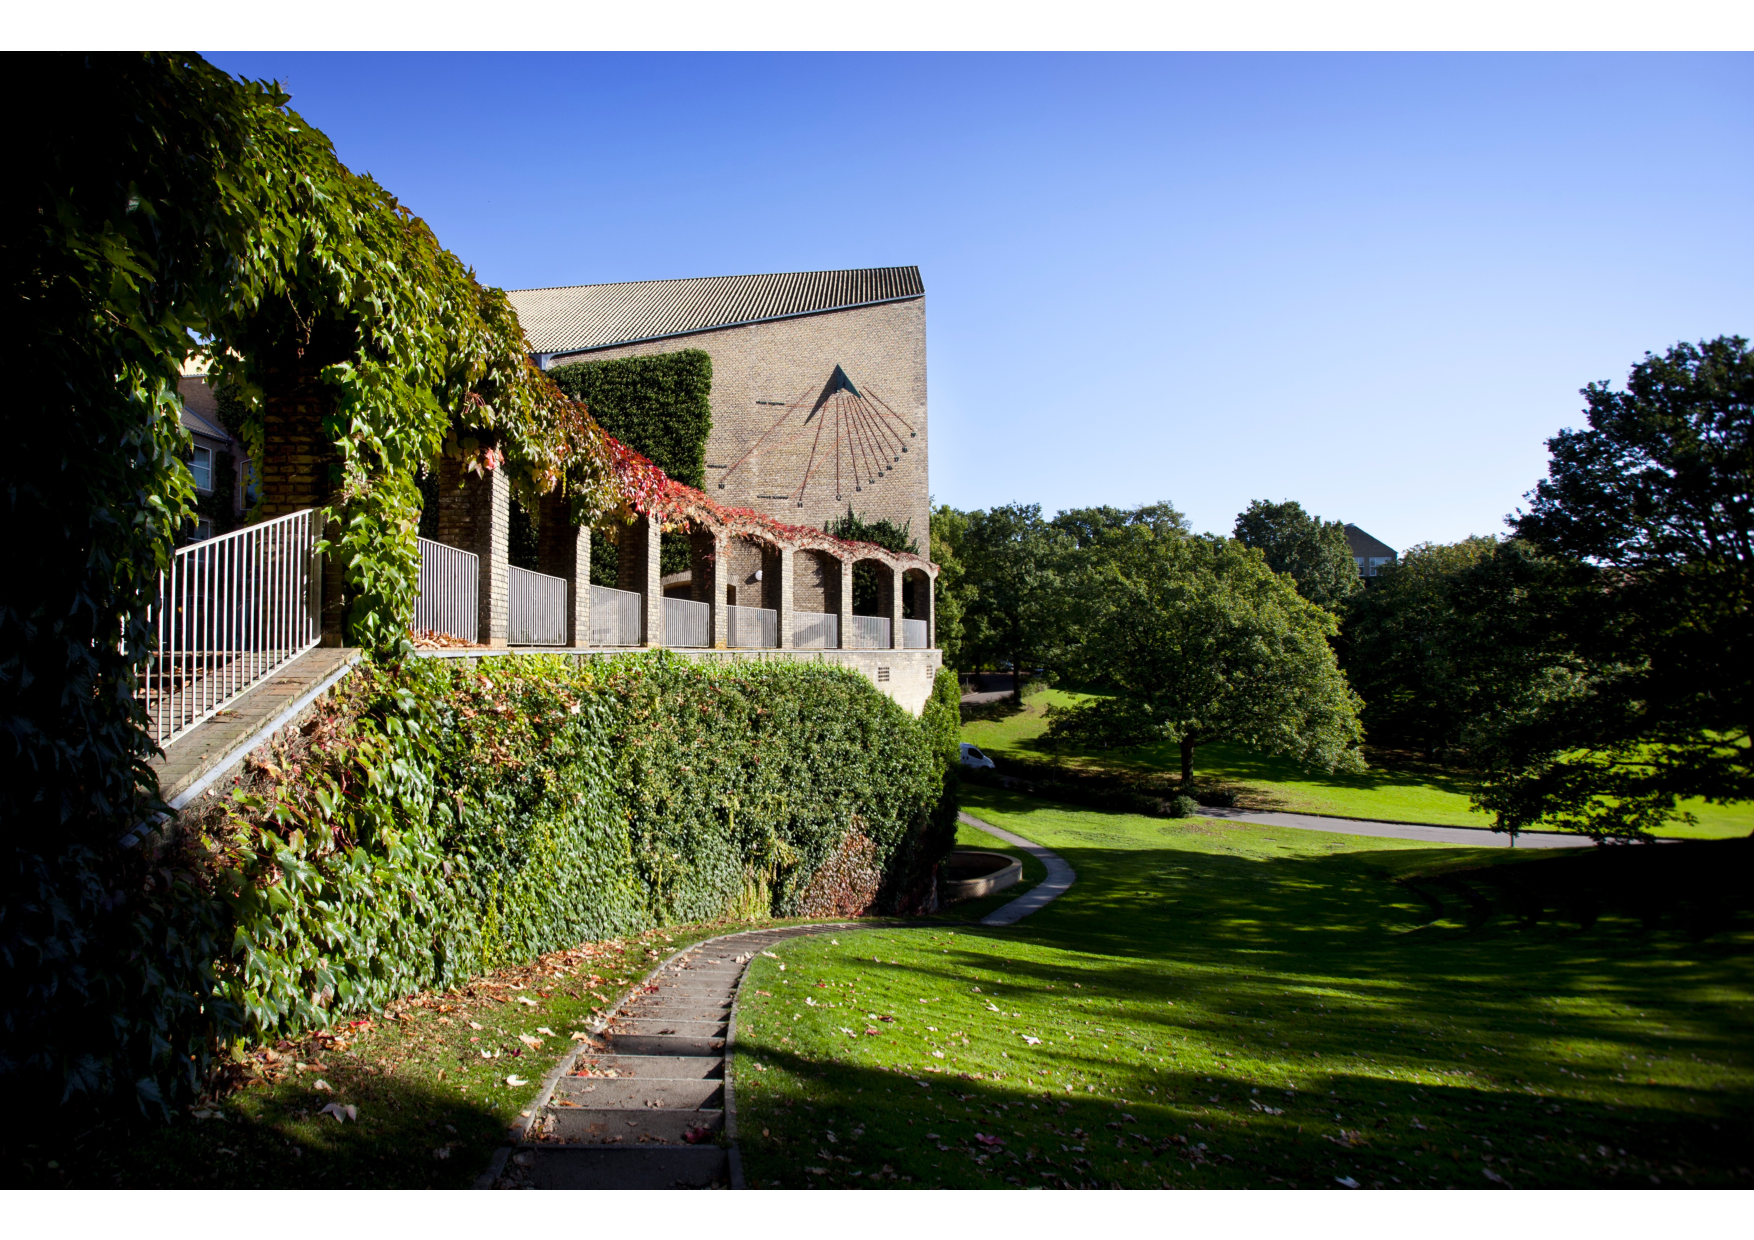
\includegraphics{highres_banner.pdf}}};
\draw (current page.center) node[inner sep=0, opacity=0.5] {\resizebox{!}{100mm}{\includegraphics{ausegl_sort.pdf}}};
% \draw (current page.center) node[bag] {  
        \draw (17, 1.7) node[bag, align=right, anchor=north east] {  
    % \mytitlefont 
    \color{titlecolor} \Large \textbf{Thesis} \\ 
    \\ 
    % \mytitlefont 
    \color{titlecolor} \Huge \textbf{\thetitle} \\ 
    \\ 
    % \mytitlefont
    \color{titlecolor} \huge \theauthor \\
    \\
    % \mytitlefont 
    \color{titlecolor} \Large \thedate 
    };
\end{tikzpicture}
\clearpage}

% back side
\AtEndDocument{\clearpage\thispagestyle{empty}
\begin{tikzpicture}[remember picture,overlay]
\draw (current page.center) node[inner sep=0] {\resizebox{!}{350mm}{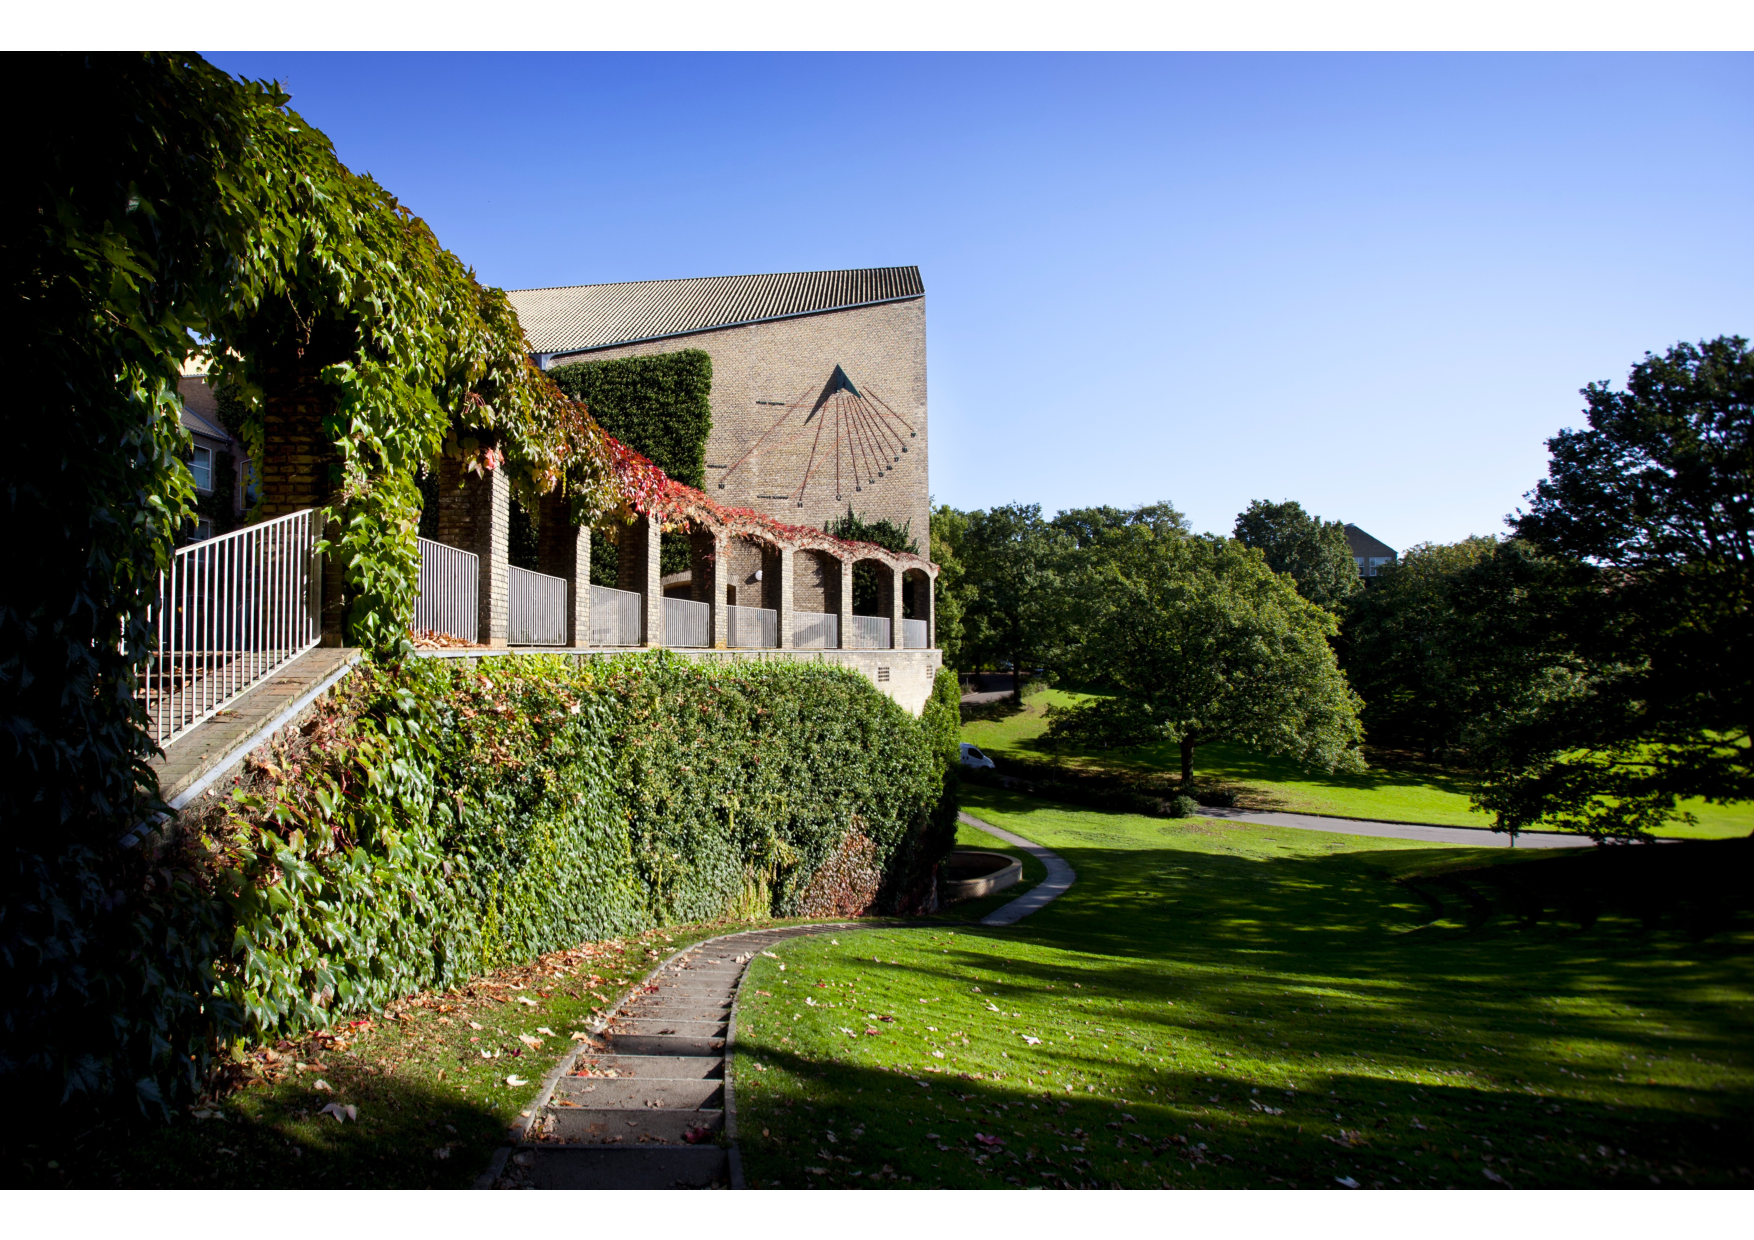
\includegraphics{highres_banner.pdf}}};
% \draw (current page.center) node[bag] {  
    \draw (17, 1.7) node[bag, align=right, anchor=north east] {  
        % \mytitlefont 
        \color{titlecolor} \large Bioinformatics Research Centre \\ 
        % \mytitlefont 
        \color{titlecolor} \large Department of Molecular Biology and Genetics \\ 
        % \mytitlefont 
        \color{titlecolor} \large Aarhus University \\
        % \mytitlefont 
        \color{titlecolor} \large Universitetsbyen 81 \\
        % \mytitlefont 
        \color{titlecolor} \large 8000 Aarhus C \\
        % \mytitlefont 
        \color{titlecolor} \large Denmark
        };

\end{tikzpicture}}


% % picture (AU logo in title page)
% \usepackage{titlepic}
% % \usepackage{graphicx}
% \titlepic{\resizebox{!}{50mm}{\includegraphics[width=\textwidth]{ausegl_sort.pdf}}}



% \pagestyle{plain} % no running header

\usepackage[many]{tcolorbox}
\definecolor{quotegray}{HTML}{505050}
\newtcolorbox{myquote}{%
    enhanced jigsaw, 
    breakable,      % allow page breaks
    frame hidden,   % hide the default frame
    left=1cm,       % left margin
    right=1cm,      % right margin
    colback=white,
    fontupper=\color{quotegray},
    overlay={%
        \node [scale=4,
            text=lightgray,
            inner sep=0pt,] at ([xshift=0.5cm,yshift=-0.7cm]frame.north west){``}; 
        \node [scale=4,
            text=lightgray,
            inner sep=0pt,] at ([xshift=-0.5cm]frame.south east){''};  
            },
        % paragraph skips obeyed within tcolorbox
                parbox=false,
}
% redefine the 'quote' environment to use this 'myquote' environment
\renewenvironment{quote}{\begin{myquote}}{\end{myquote}}

% add a dummy abstract environment that is defined in quarto manuscript 
% but not in the quarto book that we run first to give it a slot in the 
% side bar
\ifcsmacro{abstract}{}{
  \let\endmyenvironment\undefined%
  \newenvironment{abstract}{\chapter*{Abstract}}{}
}

% \usepackage{framed} % not sure i need this anymore

% \usepackage[T1]{fontenc}
% \usepackage{inconsolata}

% % I have to only define Shaded if it is already defined.
% % The reason is that pandoc does not define the macro if there are not code blocks in the a markdown file.
% \ifx \@Shaded \@empty

% \renewcommand{\KeywordTok}[1]{\textcolor[rgb]{0, 0, 0}{\textbf{{#1}}}} % def and or not reg
% \renewcommand{\BuiltInTok}[1]{\textcolor[rgb]{0.373, 0.298, 0.580}{\textbf{{#1}}}} % print open 
% \renewcommand{\VariableTok}[1]{\textcolor[rgb]{0.141, 0.392, 0.824}{\textbf{{#1}}}}
% \renewcommand{\OperatorTok}[1]{\textcolor[rgb]{0, 0, 0}{{#1}}} % def and or not reg
% \renewcommand{\DataTypeTok}[1]{\textcolor[rgb]{1.0,0.13,0.00}{{#1}}}
% \renewcommand{\DecValTok}[1]{\textcolor[rgb]{0.655, 0.498, 0.161}{{#1}}}
% \renewcommand{\BaseNTok}[1]{\textcolor[rgb]{0.259, 0.592, 0.596}{{#1}}}
% \renewcommand{\FloatTok}[1]{\textcolor[rgb]{0.655, 0.498, 0.161}{{#1}}}
% \renewcommand{\CharTok}[1]{\textcolor[rgb]{0.678,0.141,0.098}{{#1}}}
% \renewcommand{\StringTok}[1]{\textcolor[rgb]{0.678,0.141,0.098}{{#1}}}
% \renewcommand{\CommentTok}[1]{\textcolor[rgb]{0.135, 0.134, 0.133}{{#1}}}
% \renewcommand{\OtherTok}[1]{\textcolor[rgb]{0.00,0.44,0.13}{{#1}}}
% \renewcommand{\AlertTok}[1]{\textcolor[rgb]{1.00,0.00,0.00}{\textbf{{#1}}}}
% \renewcommand{\FunctionTok}[1]{\textcolor[rgb]{0.549, 0.102, 0.063}{\textbf{{#1}}}}  % function name
% \renewcommand{\RegionMarkerTok}[1]{{#1}}
% \renewcommand{\ErrorTok}[1]{\textcolor[rgb]{1.00,0.00,0.00}{\textbf{{#1}}}}
% \renewcommand{\NormalTok}[1]{\textcolor[rgb]{0, 0, 0}{{#1}}}


% \else
%   % no code blocks with markup...
% \fi



\usepackage{etoolbox}
\makeatletter
\g@addto@macro{\appendix}{%
  \patchcmd{\@@makechapterhead}% <cmd>
    {\endgraf\nobreak\vskip.5\baselineskip}% <search>
    {\hspace*{-.5em}:\space}% <replace>
    {}{}% <success><failure>
  \patchcmd{\@chapter}% <cmd>
    {\addchaptertocentry{\thechapter}}% <search>
    {\addchaptertocentry{Appendix~\thechapter:}}% <replace>
    {}{}% <success><failure>
  \addtocontents{toc}{%
    \protect\patchcmd{\protect\l@chapter}% <cmd>
      {1.5em}% <search>
      {6.5em}% <replace>
      {}{}}% <success><failure>
}
\renewcommand{\autodot}{}% Remove all end-of-counter dots
\makeatother


% restart chapter numbers in each part
\makeatletter
\@addtoreset{chapter}{part}
\makeatother


% \usepackage{chngcntr}
% \counterwithin*{subsubsection}{chapter}
% \counterwithout*{subsubsection}{section}
% \counterwithout*{subsubsection}{subsection}

% %  % KMT only use subsubsection number (this increments though the book 
% %  % when we supress numbering with  {.unnumbered} after each header except Exerisices
% \renewcommand\thesubsubsection{\arabic{section}}
% \renewcommand\thesubsubsection{\arabic{subsection}}
% \renewcommand\thesubsubsection{\arabic{chapter}-\arabic{subsubsection}}


\renewcommand*{\chapterformat}{%
  \textcolor[rgb]{0.7, 0.7, 0.7}{\thechapter}\autodot\enskip%
}
\renewcommand*{\sectionformat}{%
  \textcolor[rgb]{0.7, 0.7, 0.7}{\thesection}\autodot\enskip%
}
\renewcommand*{\subsectionformat}{%
  \textcolor[rgb]{0.7, 0.7, 0.7}{\thesubsection}\autodot\enskip%
}
\renewcommand*{\subsubsectionformat}{%
  \textcolor[rgb]{0.7, 0.7, 0.7}{\thesubsubsection}\autodot\enskip%
}



% % prevent latex from "floating" the figures
% \usepackage{float}
% \let\origfigure\figure
% \let\endorigfigure\endfigure
% \renewenvironment{figure}[1][2] {
%     \expandafter\origfigure\expandafter[H]
% } {
%     \endorigfigure
% }

\makeatletter
\@ifpackageloaded{caption}{}{\usepackage{caption}}
\AtBeginDocument{%
\ifdefined\contentsname
  \renewcommand*\contentsname{Table of contents}
\else
  \newcommand\contentsname{Table of contents}
\fi
\ifdefined\listfigurename
  \renewcommand*\listfigurename{List of Figures}
\else
  \newcommand\listfigurename{List of Figures}
\fi
\ifdefined\listtablename
  \renewcommand*\listtablename{List of Tables}
\else
  \newcommand\listtablename{List of Tables}
\fi
\ifdefined\figurename
  \renewcommand*\figurename{Figure}
\else
  \newcommand\figurename{Figure}
\fi
\ifdefined\tablename
  \renewcommand*\tablename{Table}
\else
  \newcommand\tablename{Table}
\fi
}
\@ifpackageloaded{float}{}{\usepackage{float}}
\floatstyle{ruled}
\@ifundefined{c@chapter}{\newfloat{codelisting}{h}{lop}}{\newfloat{codelisting}{h}{lop}[chapter]}
\floatname{codelisting}{Listing}
\newcommand*\listoflistings{\listof{codelisting}{List of Listings}}
\makeatother
\makeatletter
\makeatother
\makeatletter
\@ifpackageloaded{caption}{}{\usepackage{caption}}
\@ifpackageloaded{subcaption}{}{\usepackage{subcaption}}
\makeatother

\ifLuaTeX
  \usepackage{selnolig}  % disable illegal ligatures
\fi
\usepackage{bookmark}

\IfFileExists{xurl.sty}{\usepackage{xurl}}{} % add URL line breaks if available
\urlstyle{same} % disable monospaced font for URLs
\hypersetup{
  pdftitle={The most fantastic master thesis ever},
  pdfkeywords={Etiam quis, Pellentesque ante mauris, In id porta},
  hidelinks,
  pdfcreator={LaTeX via pandoc}}


\title{The most fantastic master thesis ever}
\usepackage{etoolbox}
\makeatletter
\providecommand{\subtitle}[1]{% add subtitle to \maketitle
  \apptocmd{\@title}{\par {\large #1 \par}}{}{}
}
\makeatother
\subtitle{A more elaborate title further explaining the topic}
\author{Jane Doe}
\date{November 22, 2024}

\begin{document}
\frontmatter
\cleardoublepage
\thispagestyle{empty}
{\centering
\hbox{}\vskip 0cm plus 1fill
{%\mytitlefont 
\Huge\bfseries The most fantastic master thesis ever \par}
\vspace{3ex}
{\Large\bfseries A more elaborate title further explaining the
topic \par}
\vspace{6ex}
{\Large\bfseries Jane Doe \par}
\vspace{3ex}
{\bfseries\large November 22, 2024 \par}
\vskip 0cm plus 2fill
{\resizebox{!}{50mm}{\includegraphics[width=\textwidth]{ausegl_sort.pdf}} \par}
\vskip 0cm plus 2fill
{\bfseries\large Master of Science in Bioinformatics \par}
\vspace{3ex}
%
%
{\bfseries\large Aarhus University \par}
%
\vspace{12ex}
{\small Submitted in fulfillment of the requirements
of the degree of Master of Science in Bioinformatics \par}
\pagebreak
\begin{quote}
\raggedright    
Etiam quis tortor luctus, pellentesque ante a, finibus dolor. Phasellus
in nibh et magna pulvinar malesuada. Ut nisl ex, sagittis at
sollicitudin et, sollicitudin id nunc. In id porta urna. Proin porta
dolor dolor, vel dapibus nisi lacinia in. Pellentesque ante mauris,
ornare non euismod a, fermentum ut sapien. Proin sed vehicula enim.
Etiam quis tortor luctus, pellentesque ante a, finibus dolor. Phasellus
in nibh et magna pulvinar malesuada. Ut nisl ex, sagittis at
sollicitudin et, sollicitudin id nunc. In id porta urna. Proin porta
dolor dolor, vel dapibus nisi lacinia in. Pellentesque ante mauris,
ornare non euismod a, fermentum ut sapien. Proin sed vehicula enim.
\end{quote}
}

\renewcommand*\contentsname{Table of contents}
{
\setcounter{tocdepth}{1}
\tableofcontents
}

\mainmatter
\chapter{Introduction}\label{introduction}

Vestibulum ultrices, tortor at mattis porta, odio nisi rutrum nulla, sit
amet tincidunt eros quam facilisis tellus. Fusce eleifend lectus in
elementum lacinia. Nam auctor nunc in massa ullamcorper, sit amet auctor
ante accumsan. Nam ut varius metus. Curabitur eget tristique leo. Cras
finibus euismod erat eget elementum. Integer vel placerat ex. Ut id eros
quis lectus lacinia venenatis hendrerit vel ante.

\chapter{Results}\label{results}

\begin{figure}[H]

\centering{

\includegraphics[width=3.82292in,height=2.97917in]{index_files/figure-latex/..-notebooks-example-fig-danish-interaction-output-1.png}

}

\caption{\label{fig-danish-interaction}Interaction among Danes: How
Danes interact is has very little to do with age and seniority, compared
to most other contries.}

\end{figure}%

Etiam congue quam eget velit convallis, eu sagittis orci vestibulum.
Vestibulum at massa turpis. Curabitur ornare ex sed purus vulputate,
vitae porta augue rhoncus. Phasellus auctor suscipit purus, vel
ultricies nunc. Nunc eleifend nulla ac purus volutpat, id fringilla
felis aliquet. Duis vitae porttitor nibh, in rhoncus risus. Vestibulum a
est vitae est tristique vehicula. Proin mollis justo id est tempus
hendrerit. Praesent suscipit placerat congue. Aliquam eu elit gravida,
consequat augue non, ultricies sapien. Nunc ultricies viverra ante, sit
amet vehicula ante volutpat id. Etiam tempus purus vitae tellus mollis
viverra. Donec at ornare mauris. Aliquam sodales hendrerit ornare.
Suspendisse accumsan lacinia sapien, sit amet imperdiet dui molestie ut.

\section{Subsection}\label{subsection}

\begin{figure}[H]

\centering{

\includegraphics[width=4.54167in,height=2.97917in]{index_files/figure-latex/..-notebooks-example-fig-meaninformality-output-1.png}

}

\caption{\label{fig-meaninformality}Mean interaction scores by position
and nationality.}

\end{figure}%

Table~\ref{tbl-meaninformality} lists the mean interaction scores by
position and nationality.

\begin{longtable}[]{@{}lll@{}}

\caption{\label{tbl-meaninformality}Mean interaction scores by position
and nationality.}

\tabularnewline

\caption{}\label{T_da10d}\tabularnewline
\toprule\noalign{}
position & nationality & informality \\
\midrule\noalign{}
\endfirsthead
\toprule\noalign{}
position & nationality & informality \\
\midrule\noalign{}
\endhead
\bottomrule\noalign{}
\endlastfoot
Professor & GB & 8.380414 \\
Postdoc & NL & 8.784014 \\
Postdoc & GB & 8.795308 \\
Postdoc & US & 8.826106 \\
Professor & UK & 9.360650 \\
PhDstudent & DK & 9.506580 \\
PhDstudent & UK & 10.063141 \\
Postdoc & DK & 10.279960 \\
PhDstudent & CH & 10.426218 \\
Professor & DK & 10.449005 \\

\end{longtable}

\subsection{Subsubsection}\label{subsubsection}

Duis urna urna, pellentesque eu urna ut, malesuada bibendum dolor.
Suspendisse potenti. Vivamus ornare, arcu quis molestie ultrices, magna
est accumsan augue, auctor vulputate erat quam quis neque. Nullam
scelerisque odio vel ultricies facilisis. Ut porta arcu non magna
sagittis lacinia. Cras ornare vulputate lectus a tristique. Pellentesque
ac arcu congue, rhoncus mi id, dignissim ligula.

\chapter{Methods}\label{methods}

Table~\ref{tbl-subjects} lists the samples included in the analysis.

Duis ornare ex ac iaculis pretium. Maecenas sagittis odio id erat
pharetra, sit amet consectetur quam sollicitudin. Vivamus pharetra quam
purus, nec sagittis risus pretium at. Nullam feugiat, turpis ac accumsan
interdum, sem tellus blandit neque, id vulputate diam quam semper nisl.
Donec sit amet enim at neque porttitor aliquet. Phasellus facilisis
nulla eget placerat eleifend. Vestibulum non egestas eros, eget lobortis
ipsum. Nulla rutrum massa eget enim aliquam, id porttitor erat luctus.
Nunc sagittis quis eros eu sagittis. Pellentesque dictum, erat at
pellentesque sollicitudin, justo augue pulvinar metus, quis rutrum est
mi nec felis. Vestibulum efficitur mi lorem, at elementum purus
tincidunt a. Aliquam finibus enim magna, vitae pellentesque erat
faucibus at. Nulla mauris tellus, imperdiet id lobortis et, dignissim
condimentum ipsum. Morbi nulla orci, varius at aliquet sed, facilisis id
tortor. Donec ut urna nisi.

\phantomsection\label{doc-sampling}
The 24 subjects from workplaces in Denmark were interviewed \ldots. blah
blah blah blah blah blah blah blah blah blah blah blah blah blah blah
blah blah blah blah blah blah blah blah blah blah blah blah blah blah
blah blah blah blah blah blah blah

Ut ut condimentum augue, nec eleifend nisl. Sed facilisis egestas odio
ac pretium. Pellentesque consequat magna sed venenatis sagittis. Vivamus
feugiat lobortis magna vitae accumsan. Pellentesque euismod malesuada
hendrerit. Ut non mauris non arcu condimentum sodales vitae vitae dolor.
Nullam dapibus, velit eget lacinia rutrum, ipsum justo malesuada odio,
et lobortis sapien magna vel lacus. Nulla purus neque, hendrerit non
malesuada eget, mattis vel erat. Suspendisse potenti.

\begin{longtable}[]{@{}lllll@{}}

\caption{\label{tbl-subjects}People included in the analysis.}

\tabularnewline

\caption{}\label{T_e468d}\tabularnewline
\toprule\noalign{}
name & age & sex & position & nationality \\
\midrule\noalign{}
\endfirsthead
\toprule\noalign{}
name & age & sex & position & nationality \\
\midrule\noalign{}
\endhead
\bottomrule\noalign{}
\endlastfoot
Julie & 27 & F & PhDstudent & DK \\
Thomas & 33 & M & Postdoc & GB \\
Emilie & 23 & F & PhDstudent & CH \\
Sofie & 31 & F & Postdoc & DK \\
Sara & 29 & F & Postdoc & US \\
Cecilie & 34 & F & Postdoc & DK \\
Anders & 32 & M & PhDstudent & UK \\
Emma & 42 & F & Professor & DK \\
Caroline & 31 & F & PhDstudent & DK \\
Laura & 30 & F & Postdoc & DK \\
Mikkel & 33 & M & Postdoc & NL \\
Jens & 27 & M & PhDstudent & DK \\
Andreas & 29 & M & PhDstudent & DK \\
Jakob & 28 & M & PhDstudent & DK \\
Mathilde & 61 & F & Professor & DK \\
Katrine & 35 & F & Postdoc & DK \\
Poul & 30 & M & Postdoc & DK \\
Anna & 26 & F & PhDstudent & DK \\
Peter & 42 & M & Professor & GB \\
Ida & 53 & F & Postdoc & DK \\
Freja & 30 & F & Postdoc & DK \\
Maria & 39 & F & Professor & UK \\
Amalie & 29 & F & PhDstudent & DK \\
Camilla & 35 & F & Postdoc & DK \\

\end{longtable}

Nullam dapibus cursus dolor sit amet consequat. Nulla facilisi.
Curabitur vel nulla non magna lacinia tincidunt. Duis porttitor quam
leo, et blandit velit efficitur ut. Etiam auctor tincidunt porttitor.
Phasellus sed accumsan mi. Fusce ut erat dui. Suspendisse eu augue eget
turpis condimentum finibus eu non lorem. Donec finibus eros eu ante
condimentum, sed pharetra sapien sagittis. Phasellus non dolor ac ante
mollis auctor nec et sapien. Pellentesque vulputate at nisi eu
tincidunt. Vestibulum at dolor aliquam, hendrerit purus eu, eleifend
massa. Morbi consectetur eros id tincidunt gravida. Fusce ut enim quis
orci hendrerit lacinia sed vitae enim.

\chapter{Bon mot}\label{bon-mot}

\begin{quote}
Nothing in Biology Makes Sense except in the Light of Evolution

- Theodosius Dobzhansky
\end{quote}


\backmatter


\end{document}
